\section{Exercice 3.4 Single frequency pos. effects}


\textcolor{red}{añadir NEU al glosario}\\
Exercise: Analyze the single frequency positioning solution under the Halloween storm.

The following steps are recommended:
\begin{enumerate}
\item Using files amc23020.03o,brdc3030.03n compute with gLAB the following solutions:
    \begin{enumerate}
        \item Solution with full SPS modeling. Name output file as: gLAB.out
        \item Solution with the ionospheric corrections disabled: gLAB1.out
        \item Solution with the 2-freq. Ionosphere-free code (PC): gLAB2.out
    \end{enumerate}
\item Plot results
\end{enumerate}

\begin{figure}[H]
        \centering
        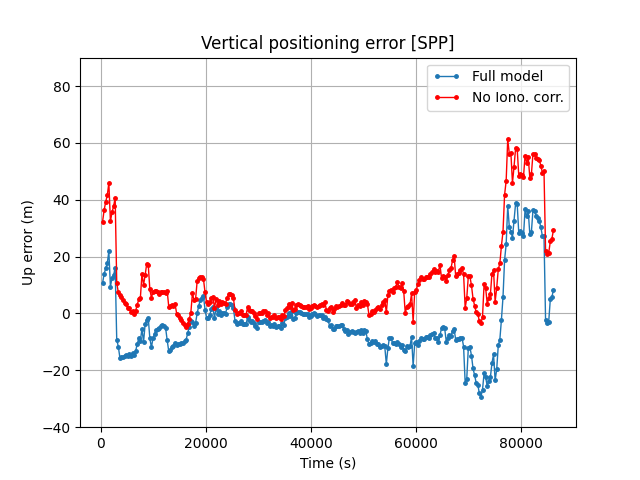
\includegraphics[scale=0.52]{sources/Figures/FIG_2/TUT2_Ex3.4.2c.png}
        \caption{NEU SPP full model with (Klobuchar)}
        \label{fig:NEU SPP full model with (Klobuchar)}
\end{figure}


\begin{figure}[H]
        \centering
        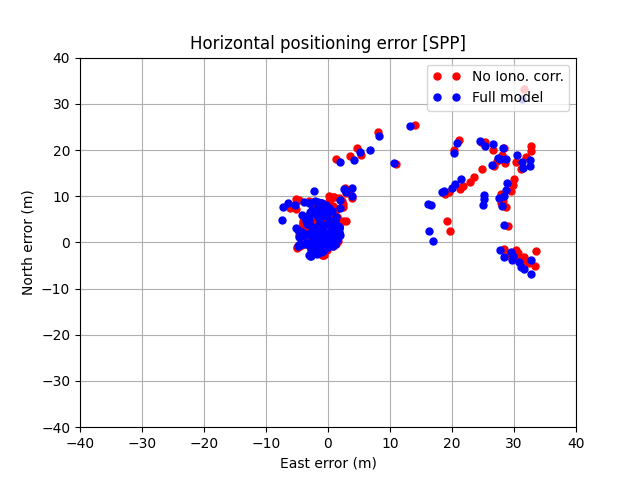
\includegraphics[scale=0.52]{sources/Figures/FIG_2/TUT2_Ex3.4.2d.png}
        \caption{}
        \label{}
\end{figure}


\begin{figure}[H]
        \centering
        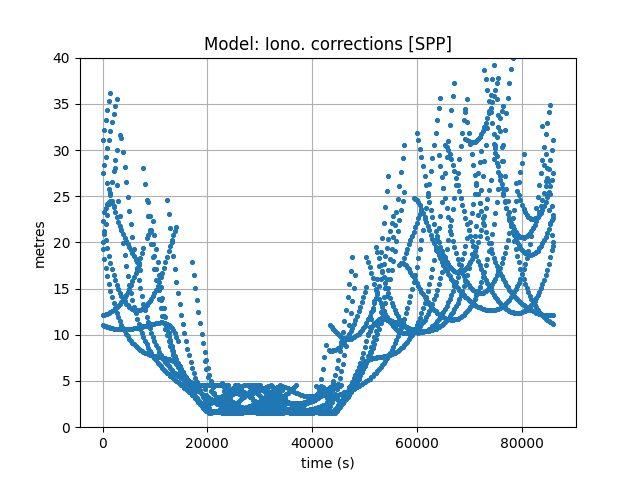
\includegraphics[scale=0.52]{sources/Figures/FIG_2/TUT2_Ex3.4.2e.png}
        \caption{}
        \label{}
\end{figure}


\begin{figure}[H]
        \centering
        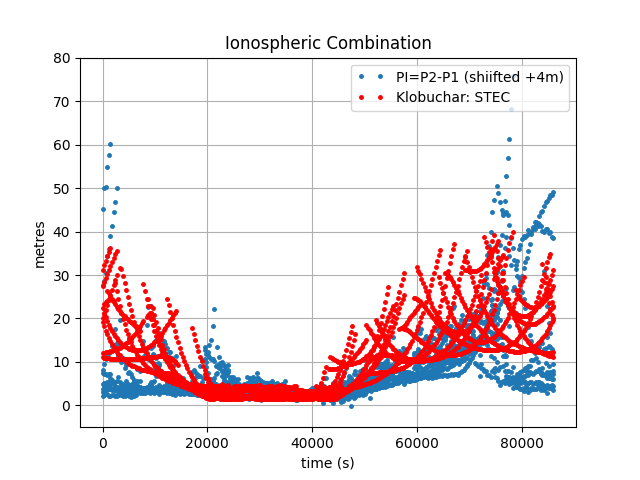
\includegraphics[scale=0.52]{sources/Figures/FIG_2/TUT2_Ex3.4.2f.png}
        \caption{}
        \label{}
\end{figure}